% Updated in May 2014 by Hideo Saito
% Updated in March 2012 by Yasuyuki Matsushita
% Updated in April 2002 by Antje Endemann, ...., and in March 2010 by Reinhard Klette
% Based on CVPR 07 and LNCS style, with modifications by DAF, AZ and elle 2008, AA 2010, ACCV 2010

\documentclass[runningheads]{llncs}
\usepackage{graphicx}
\usepackage{amsmath,amssymb} % define this before the line numbering.
\usepackage{ruler}
\usepackage{color}

\usepackage{epstopdf}
\usepackage{times}
\usepackage{epsfig}
\usepackage{graphicx}
\usepackage{url}
\usepackage{bm}

%===========================================================
\begin{document}
\pagestyle{headings}
\mainmatter


\def\ACCV14SubNumber{215}  % Insert your submission number here

%===========================================================
\title{Clouds in The Cloud\\
Supplementary Material}
\titlerunning{ACCV-14 submission ID \ACCV14SubNumber - Supplementary Material}
\authorrunning{ACCV-14 submission ID \ACCV14SubNumber - Supplementary Material}

\author{Anonymous ACCV 2014 submission}
\institute{Paper ID \ACCV14SubNumber}

\maketitle

%===========================================================
\section{Simulations}

We used simulated data to test the camera network concept
quantitatively and to scale it to large number of cameras. In this
section we detail the simulation setup and results.

% -------------------------------------------------------------------------
\subsection{Setup}

Quantitative assessments used atmospheric-science gold standard
simulators.  An atmosphere over $8\times8{\rm km}$ was produced using
off-the-shelf large eddy simulation (LES), creating clouds between
heights of $500{\rm m}$ to $1500{\rm m}$.  Lighting conditions were
consistent with Copenhagen (unrelated to the anonymous authors).
Radiative transfer using the discrete ordinate spherical-harmonic
method (SHDOM)~\cite{Evans1998} rendered images taken by 100 cameras
placed in a $2.5\times 2.5{\rm km}^2$ domain. Recovery simulations
used random subsets of the network, where the whole network is either
with or without a sun blocker. In the LES, a voxel is occupied by
cloud if its water-mass parameter is not null. In the recovery, voxel
$k$ is classified as cloud if $T_k>0.01$.  We measured the
classification error rate, across all voxels.
% Note that the LES example details the water particle distribution
% and therefore $B$ is calculated as the voxels where the water
% content equals are surpasses some threshold.  The threshold we used
% was half the maximal water content in the example.  Due to this
% method we don't expect to achieve perfect reconstruction.
The results are plotted in Fig.~\ref{fig:simulations}.  As expected of
space carving, results improve fast from 2 to 10 cameras. Even when a
sun blocker is applied, the algorithm is able to reconstruct the cloud
formation. Then, as expected, more cameras are needed in order to
compensate for the limited view of each camera. In our setup the
cameras observe the clouds only from below. This is the classical
limited angle problem known from visual hull and tomography
algorithms. Therefore the reconstruction error does not converge to
zero.

% -------------------------------------------------------------------------
\subsection{Results}

\begin{figure}
  \begin{center}
    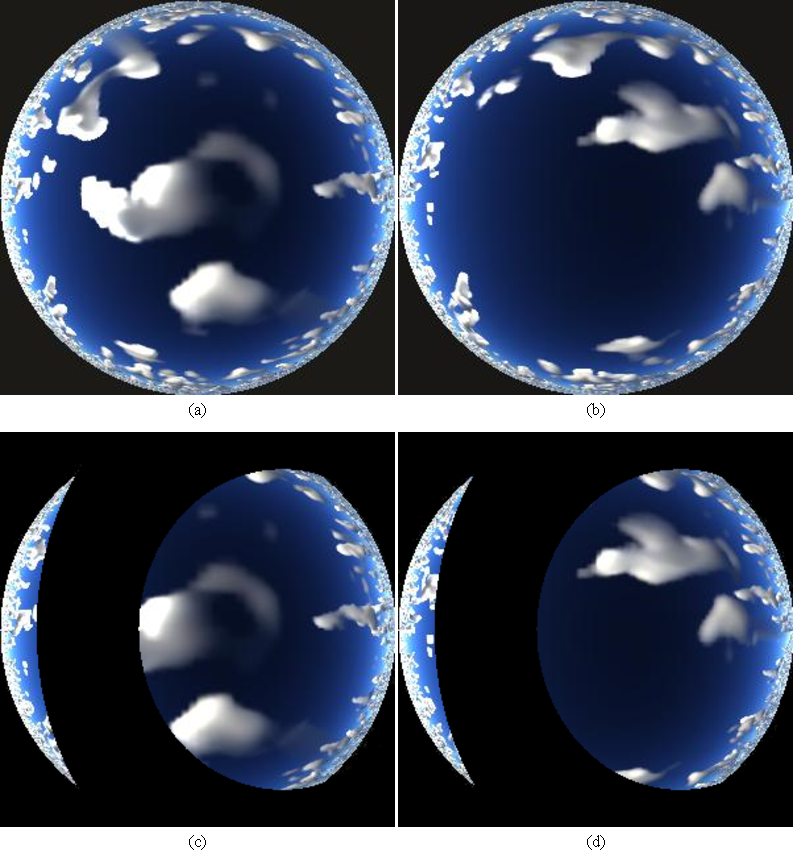
\includegraphics{figures/simulation_imgs}
    \caption{Images synthesised using SHDOM and used in the
      reconstruction algorithm.  (a,b) Images of the same scene from
      different cameras. The red rectangle marks the region of
      interest of the reconstruction algorithm. (c,d) The same images
      with the simulated sun-blocker applied.}
    \label{fig:simulation_imgs1}
  \end{center}
\end{figure}

\begin{figure}
  \begin{center}
    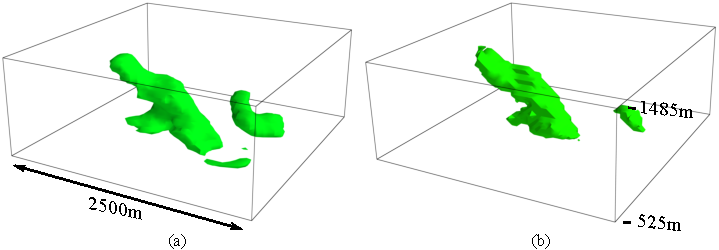
\includegraphics{figures/clouds3d_SHDOM}
    \caption{Simulated clouds.}
    \label{fig:simulation_imgs2}
  \end{center}
\end{figure}

\begin{figure}
  \begin{center}
    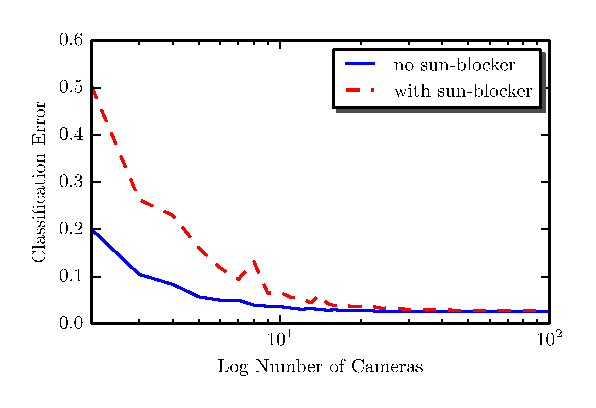
\includegraphics{figures/simulations.eps}
    \caption{Classification error rate as a function of the number of
      cameras. [Solid Blue] Without sun blocker. [Dashed Red] With sun
      blocker.  Fluctuations are within the random sampling standard
      deviation.}
    \label{fig:simulation}
  \end{center}
\end{figure}


% ===========================================================
\section{SIFT}

%%%%%%%%%%%%%%%%%%%%%%%%%%%%%%%%%%%%%%%%%%%%%%%%%%%%%%%%%%%%%%
\subsection*{Spatial similarity score}
\label{sec:appearancecore}

During our experiments, we had found that simple color consistency was not enough when tackling difficult cloud structures such as high-altitude ciruss due to spatial ambiguity and very low baseline between the cameras. In such cases spatial information would be a natural way of incorporating a multi-view stereo approach into our space-carving scheme.
To this end, we introduce an additional score-function $\{S_k\}$ which promotes  structural similarity between patches around the projected voxel.
Dense SIFT~\cite{DenseSift2011} has recently been proven to be an efficient feature for non-rigid matching between pairs of images.
In a similar manner, dense SIFT can be incorporated in our probablistic Space-Carving scheme together with the calor values to represent the appearance of a pgojected voxel. SIFT descriptors also give us the benefit of robustness under scale and view-angle variations.
As in ~\cite{DenseSift2011}, 128-bin dense SIFT descriptors were chosen.
Per voxel $k$, the set of measured radiances is \mbox{${\cal I}_t(k)\equiv\{\hat I_t(r)\}_{r\in\rho_k}$}. Across viewpoints, the measured variance of this set is ${\rm VAR}[{\cal I}_t(k)]$, per $t$. We define the spatial similarity score in a similar manner as was defined for the photo-consistency in Eq.10:
\begin{equation}
 P_k= \exp\left(
         -\Sigma_{\rm bin}\{{\rm VAR}[{\cal SIFT}_t^{\rm bin}(k)]\}/\sigma'^2
         \right)
  \;,
 \label{eq:Dist}
\end{equation}
where $\sigma'^2$ is a scale parameter, and $bin=\{1..128\}$. ${\rm VAR}[{\cal SIFT}_t^{\rm bin}(k)]$ computes the variance at each bin. Overall, the total cloud-score of a voxel is $T_k=B_kP_k$.
Figure ... shows the reconstruction with and without the SIFT 





%===========================================================
\bibliographystyle{splncs}
\bibliography{cloudsbib}

%this would normally be the end of your paper, but you may also have an appendix
%within the given limit of number of pages
\end{document}
